% Copyright 2004 by Till Tantau <tantau@users.sourceforge.net>.
%
% In principle, this file can be redistributed and/or modified under
% the terms of the GNU Public License, version 2.
%
% However, this file is supposed to be a template to be modified
% for your own needs. For this reason, if you use this file as a
% template and not specifically distribute it as part of a another
% package/program, I grant the extra permission to freely copy and
% modify this file as you see fit and even to delete this copyright
% notice. 

\documentclass{beamer}

% There are many different themes available for Beamer. A comprehensive
% list with examples is given here:
% http://deic.uab.es/~iblanes/beamer_gallery/index_by_theme.html
% You can uncomment the themes below if you would like to use a different
% one:

\usetheme{Singapore}
\usecolortheme{orchid}
\setbeamerfont{block body}{size=\footnotesize}

\usepackage[T1]{fontenc}
\usepackage{amsfonts}       % blackboard math symbols
\usepackage{nicefrac}       % compact symbols for 1/2, etc.
\usepackage{amsmath}
\usepackage{latexsym}
\usepackage{amssymb}
\usepackage{mathtools}
\usepackage{graphicx}
\usepackage{booktabs}
\usepackage{tabularx}
\usepackage{bm}
\usepackage{subfig}
\usepackage{array}
\usepackage{caption}
\usepackage{natbib}

\bibliographystyle{abbrvnat}

\DeclareMathOperator*{\argmax}{\arg\max}
\DeclareMathOperator*{\argmin}{\arg\min}
\DeclareMathOperator*{\E}{\mathbb{E}}

\newcommand{\diag}[0]{\operatorname{diag}}
\newcommand{\vect}[1]{\mathbf{#1}}
\newcommand{\vects}[1]{\boldsymbol{#1}}
\newcommand{\matr}[1]{\mathbf{#1}}
\newcommand{\matrs}[1]{\boldsymbol{#1}}

\newcommand{\va}[0]{\vect{a}}
\newcommand{\vh}[0]{\vect{h}}
\newcommand{\vn}[0]{\vect{n}}
\newcommand{\vq}[0]{\vect{q}}
\newcommand{\vs}[0]{\vect{s}}
\newcommand{\vu}[0]{\vect{u}}
\newcommand{\vw}[0]{\vect{w}}
\newcommand{\vx}[0]{\vect{x}}
\newcommand{\vz}[0]{\vect{z}}

\newcommand{\mA}[0]{\matr{A}}
\newcommand{\mE}[0]{\matr{E}}
\newcommand{\mN}[0]{\matr{N}}
\newcommand{\mS}[0]{\matr{S}}
\newcommand{\mW}[0]{\matr{W}}
\newcommand{\mX}[0]{\matr{X}}

\graphicspath{{../report/images/}}

\title{Rare Event Simulation using Interacting Particle Systems for Rare Credit Portfolio Losses}

\author{
  Abhishek Shah \\
  \and
  Prithvi Krishna Gattamaneni\\
  \and
  Raghav Singhal\\
  \and
  Srivas Venkatesh \\
}
% - Give the names in the same order as the appear in the paper.
% - Use the \inst{?} command only if the authors have different
%   affiliation.

\institute[New York University] % (optional, but mostly needed)
{
  Courant Institute of Mathematical Sciences\\
  New York University\\
}
% - Use the \inst command only if there are several affiliations.
% - Keep it simple, no one is interested in your street address.

\date{\today}
% - Either use conference name or its abbreviation.
% - Not really informative to the audience, more for people (including
%   yourself) who are reading the slides online

\subject{Rare Event Simulation using Interacting Particle Systems for Rare Credit Portfolio Losses}
% This is only inserted into the PDF information catalog. Can be left
% out. 

% If you have a file called "university-logo-filename.xxx", where xxx
% is a graphic format that can be processed by latex or pdflatex,
% resp., then you can add a logo as follows:

% \pgfdeclareimage[height=0.5cm]{university-logo}{university-logo-filename}
% \logo{\pgfuseimage{university-logo}}

% Delete this, if you do not want the table of contents to pop up at
% the beginning of each subsection:
\AtBeginSubsection[]
{
  \begin{frame}<beamer>{Outline}
    \tableofcontents[currentsection,currentsubsection]
  \end{frame}
}

% Let's get started
\begin{document}

\begin{frame}
	\titlepage
\end{frame}


\begin{frame}{Outline}
	The goal of our project is to highlight IPS models for rare event siulation
	and estimation specifically in the context of Credit portfolio defaults.
																
	To that effect we talk about the following:
	\begin{itemize}
		\item Interacting particle systems.
		\item Markovian intensity model of credit risk.
		\item Merton's model of credit risk.
		      \begin{itemize}
		      	\item We use an adapted model with stochastic volatility which
		      	      is explained later.
		      \end{itemize}
	\end{itemize}
\end{frame}

\begin{frame}{Outline}
	\tableofcontents
	% You might wish to add the option [pausesections]
\end{frame}

% Section and subsections will appear in the presentation overview
% and table of contents.
\section{Interacting Particle Systems}
\section{Markovian Intensity models}
\section{Merton's model}
\subsection{Theory}
\begin{frame}{Credit Portfolio Model}
	\begin{itemize}
		\item Model is based on a modified version Merton's model with the
		      addition of a stochastic volatility term.
		\item We consider $N$ assets in a portfolio each with a price $S_i(t)$
		      at time $t$.
	\end{itemize}
	\begin{block}{Asset Evolution}
		\begin{equation*}
			dS_{i}(t) = rS_{i}(t)dt + \sigma_{i}\sigma(t)S_{i}(t)dW_{i}(t)
		\end{equation*}
		$r$ - risk free interest rate, $\sigma_i$ - Idiosyncratic volatility,
		$W$ - Weiner process with the following correlation structure
		\begin{equation*}
			d \langle W_{i}, W_{j} \rangle_{t} = \rho_{ij}dt
		\end{equation*}
		The stochastic volatility $\sigma(t)$ evolves according to the SDE,
		correlation structure
		\begin{equation*}
			\begin{split}
				d\sigma(t) &= \kappa(\bar{\sigma} - \sigma(t)) dt + \gamma \sqrt{\sigma(t)} dW(t) \\
				d \langle W_{i}, W \rangle_{t} &= \rho_{\sigma}dt
			\end{split}
		\end{equation*}
	\end{block}
\end{frame}

\begin{frame}{Model Implementation}
	\begin{block}{Markov Chain State}
		\begin{equation*}
			X_{n} = \left( \sigma \left( n \Delta t \right), \left( S_i \left( n \Delta
			t\right) \right)_{1 \leq i \leq N} , \min_{0 \leq m \leq n} \left( \left( S_i
			\left( m \Delta t \right) \right) \right) \right)
		\end{equation*}
	\end{block}
	\begin{itemize}
		\item State $X_n$ is $2N+1$ dimensional.
		\item Asset evolution done using Euler method with timestep granularity
		      $\delta t$.
		\item For default condition we use a barrier price $B_i$ going below
		      which is treated as a default.
		\item To increase sampling of these rare events we use IPS methodology
		      with the potential function $G_{p}(Y_{p}) = \exp[-\alpha (V(X_p) -
		      V(X_{p-1}))]$ where $V(X_p) = \sum_{i=1}^N \log (min_{0\leq m
		      	\leq p}S_{i}(m \Delta t))$.
	\end{itemize}
\end{frame}

\subsection{IPS Adaptation}
\begin{frame}{Stages of IPS}
	\begin{itemize}
		\item Involves 4 stages of operations.
		\item Initialization of price, volatility.
		\item $n$ loops of:
		      \begin{itemize}
		      	\item Selection stage to select paths that could lead to the
		      	      rare event of higher defaults.
		      	\item Mutation stage to evolve the selected paths as per the
		      	      SDEs.
		      \end{itemize}
		\item Termination stage to collect result of previous stage and estimate
		      default probabilities.
	\end{itemize}
\end{frame}

\begin{frame}{Initialization}
	\begin{block}{Initial Value}
		\begin{equation*}
			\begin{split}
				\hat{X}_0^{(j)} &= \left( \sigma(0), S_1(0), \cdots, S_N(0), S_1(0), \cdots, S_n(0) \right),  \quad 
				\forall 1 \leq j\leq M                                                                    \\
				\hat{W}_0^{(j)} &= \hat{X}_0^{(j)}
			\end{split}
		\end{equation*}
	\end{block}
	\begin{itemize}
		\item All $M$ portfolios are started with the same price and volatility.
		\item Initial minimum is same as initial price.
		\item Initial history is same as current initialization.
	\end{itemize}
\end{frame}

\begin{frame}{Selection}
	\begin{itemize}
		\item Resample with replacement $M$ paths from input $M$ paths according
		      to empirical distribution under the given Gibbs measure.
		\item $\left( \hat{W}_p^{(j)}, \hat{X}_p^{(j)} \right)$ becomes $\left( \breve{W}_p^{(j)}, \breve{X}_p^{(j)}\right)$.
	\end{itemize}
	\begin{block}{Empirical distribution}
		\begin{equation*}
			\begin{split}
				&\eta_{p}^{M}(dW,dX) = \frac{1}{M \hat{\eta}_{p}^{M}}\sum_{j=1}^{M}\exp\left[{\alpha(V(\hat{X}_{p}^{(j)}))-V(\hat{W}^{(j)}_{p})}\right] \times \delta_{(\hat{W}_p^{j},\hat{X}_p^{j})}(dW,dX) \\
				&\text{Where}\\
				&\hat{\eta}_{p}^{M} =
				\frac{1}{M}\sum_{j=1}^{M}\exp\left[{\alpha(V(\hat{X}_{p}^{(j)}))-V(\hat{W}^{(j)}_{p})}\right]
			\end{split}
		\end{equation*}
	\end{block}
\end{frame}

\begin{frame}{Mutation}
	\begin{itemize}
		\item Evolve paths from $\breve{X}_p^{(j)}$ to $\hat{X}_{p+1}^{(j)}$.
		\item Set $\hat{W}_{p+1}^{(j)} = \breve{X}_p^{(j)}$.
		\item Evolve based on SDEs using Euler-Maruyama method with time step
		      $\delta t$. Evolution is from $t_p$ to $t_{p+1}$ ($t_p + \Delta t$).
		\item $\delta t \ll \Delta t$
		\item True Dynamics.
	\end{itemize}
\end{frame}

\begin{frame}{Termination}
	\begin{itemize}
		\item Teminate at maturity time $T$ by running the selection, mutation
		      step $n$ times. ($n \Delta t = T$)
		\item Estimate default probability $p_k(T) = \mathbb{P}\left( L\left( T \right) = k
		      \right)$ using formula below.
	\end{itemize}
	\begin{block}{Estimation}
		\begin{equation*}
			\begin{split}
				&\hat{p}_{k}^{M}(T) = \left[ \frac{1}{M} \sum_{j=1}^{M} \mathbf{1}_{\lbrace f(\hat{X}_{n}^{(j)}) = k\rbrace
						}\exp\left[{\alpha(V(\hat{W}^{(j)}) - V(\hat{X_{0}}))}\right]\right] \times \left[ \prod_{p=0}^{n-1} \hat{\eta}_{p}^{M}\right] \\
						&\text{Where}\\
						&f(X^{(j)}_n) = \sum_{i=1}^{N}\mathbf{1}_{\lbrace X^{(j)}_{n}(N + 1 + i)\leq B_{i}\rbrace}
					\end{split}
				\end{equation*}
			\end{block}
		\end{frame}

\subsection{Results}
\begin{frame}{Plots}
	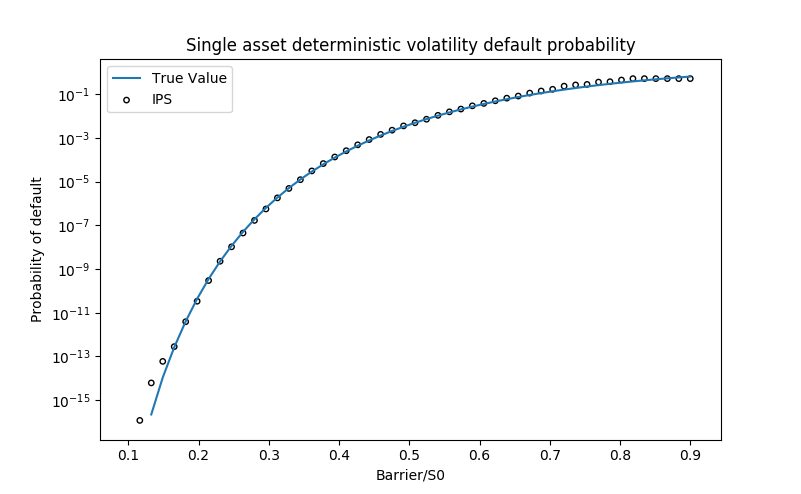
\includegraphics[width = \textwidth]{IPS_single}
\end{frame}

\begin{frame}{Plots}
	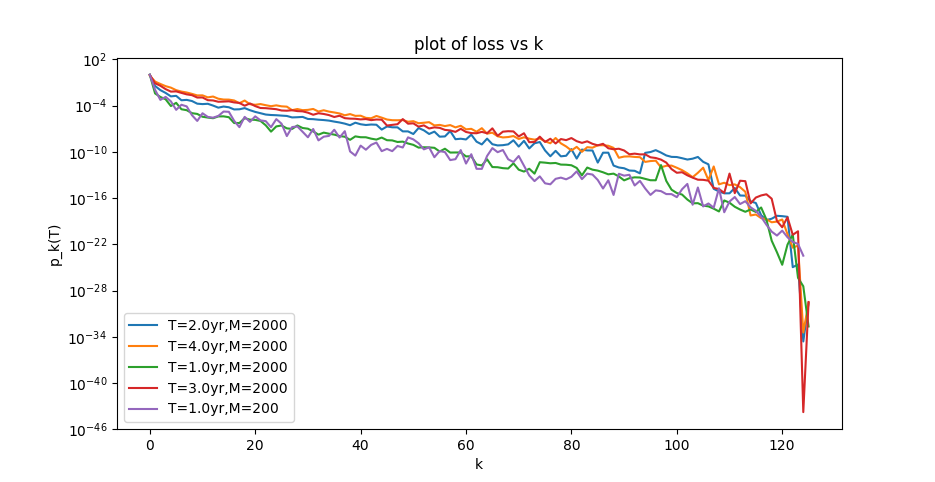
\includegraphics[width = \textwidth]{IPS_all_years}
\end{frame}

\begin{frame}{Plots}
	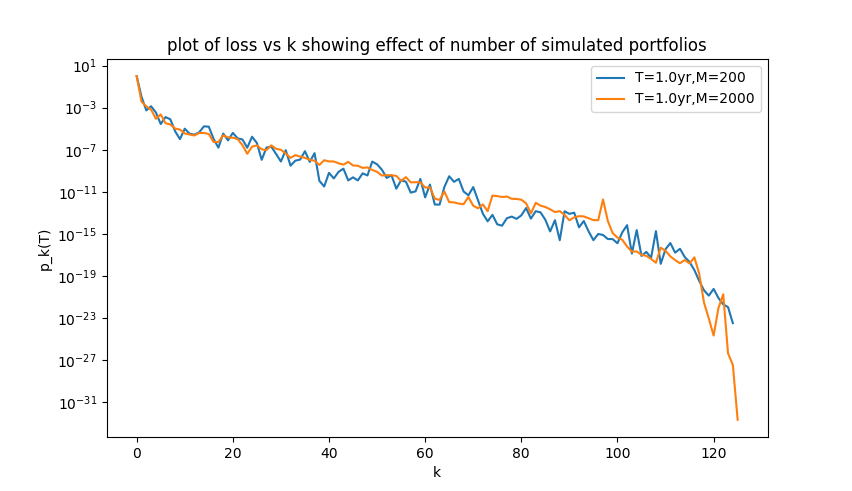
\includegraphics[width = \textwidth]{IPS_M_comparison}
\end{frame}

\begin{frame}{Plots}
	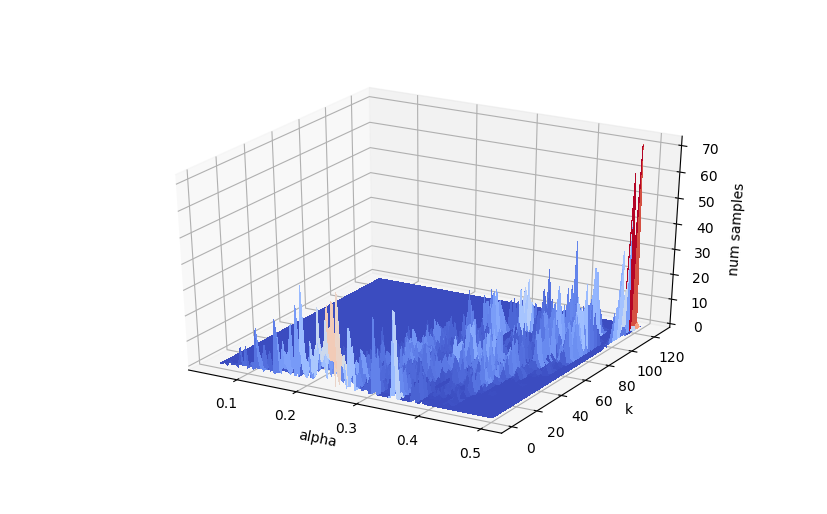
\includegraphics[width = \textwidth]{IPS_surface}
\end{frame}



% All of the following is optional and typically not needed. 
\appendix
\section<presentation>*{\appendixname}
\subsection<presentation>*{References}

\begin{frame}[allowframebreaks]
	\frametitle<presentation>{References}
													    
	\small
	\nocite{*}
	\bibliography{../report/references}
\end{frame}

\begin{frame}
	\centering
	Thank you!
													
	\huge
	Questions?
\end{frame}
\end{document}
